

Results of the time reallocation method are shown in Fig.~\ref{fig:snrCompare} and Fig.~\ref{fig:obsTimes}.
In Fig.~\ref{fig:snrCompare}, the average SNR over a $10\,{\rm yr}$ PTA lifespan is shown. 
The original observation stragegy is shown by the blue-solid line.
The results of time shuffling with three different correlation functions are shown: Hellings-Downs (orange-dot), dipole minus Hellings-Downs (green-dash), and equal (red-dot-dash).
We note that these alternative correlations functions are only used during the time-reallocation calculation, and Fig.~\ref{fig:snrCompare} shows the SNR value computed using the Hellings-Downs function as in Eqn.~\ref{eqn:snrPIPJPg}).
The gains are all less than X\% at $10\,{\rm yr}$, indicating that the current observation strategey of timing all pulsars to $1\,{\rm \mu s}$ precision is already performing well. 


Figure~\ref{fig:obsTimes} shows the corresponding integration times for the PTAs configurations shown in Fig.~\ref{fig:snrCompare}.
The different correlation function does make a difference in which pulsars gain and lose time, however we do see that it can be advantageous to reduce integration time allocated to pulsars which require more than $1500\,{\rm s}$ to achieve $1\,{\rm \mu s}$ precision. 


We see from Fig.~\ref{fig:snrCompare}, that using the Hellings-Downs function for time-reallocation provides the largest improvement in SNR (\% at 10 yr). 
However, as discussed in Section~\ref{sec:timeshuffle}, it comes at the cost of reducing the integration time for pulsar pairs with high angular separations, which could make confirming a Hellings-Downs correlation more challenging. 
This effect is clear fromt eh sky map shown in Fig.~\ref{fig:skyHD}. 
Cross markers represent each pulsar and changes in integratoin time (compared to the original strategy) are shown by circles. 
Pulsars that gain integration time are shown in orange and those that lose it in blue. 
The size of the circle is proportional to the amount of time gained or lost. 
The general trend we see is that pulsars close to the galactic centre gain time and those away from it lose time. 

The other two correlation functions we use are shown in Figs.~\ref{fig:skyDPHDDiff} and~\ref{fig:skyEqual} for dipole minus Hellings-Downs and equal correlation functions, respectively. 
In both cases, we observe less of a bias towards pulsars in the galactic centre than is seen in Fig.~\ref{fig:skyHD}.

Therefore, although using a Hellings-Downs correlation function provides the largest SNR increase in Fig.~\ref{fig:snrCompare}, we recommend replacing it with an equal-calued correlation function for the time reallocatoin calculation to prevent preference for pulsar pairs with small angular separations. 

We can also compute PTA sensitivity curves for the four configurations using \texttt{hasasia}[add ref]. 
Figure~\ref{fig:hasasia} shows the characteristic strain sensitivity for the PTAs against frequency for a $10\, {\rm yr}$ PTA using a constant cadence $c=26\,{\rm yr}^{-1}$. 
The curves include spin noise, but not jitter noise. 
A small increase in sensitivity can be seen in comparison to the original observing strategy, however the difference is minimal with $\approx 0.5 \times 10^{-16}$ difference at the most sensitive frequency (shown by the zoom inset). 
 




\begin{figure}
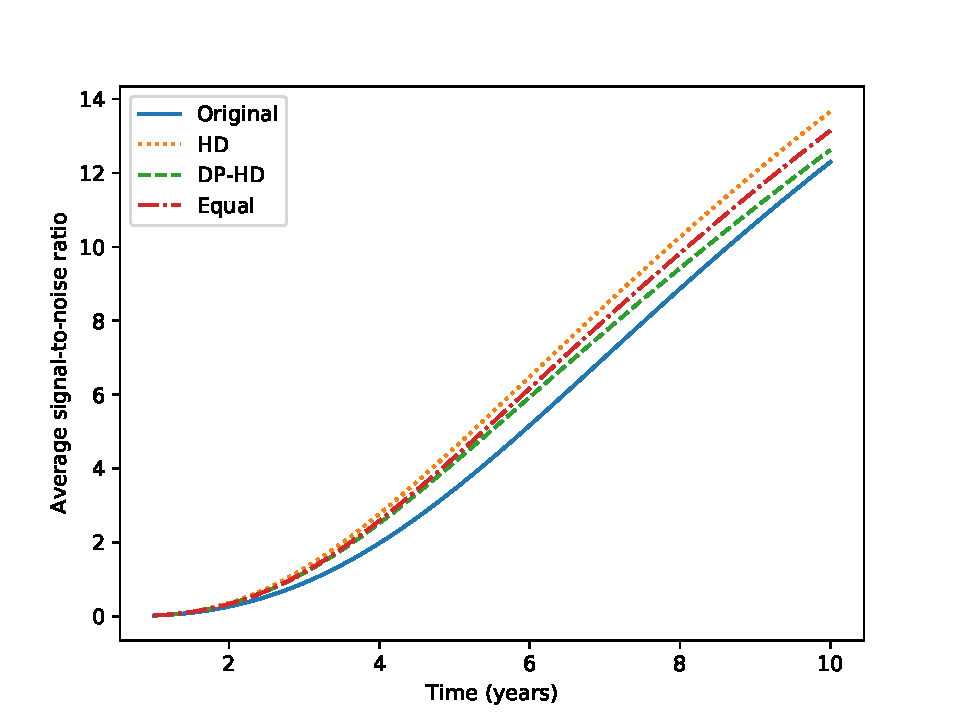
\includegraphics[width=0.5\textwidth]{./images/compareSNRVTime.pdf}
\caption{\label{fig:snrCompare}
SNR over PTA lifespan ($T$) assuming four different observation time allocations. 
Blue-solid shows the original MeerTime observing strategy.
Three time realocation results are shown, which each assume a different function for $\chiIJhd$. 
`hd' is Hellings-Downs, `dphdDiff' is the difference between dipole and Hellings-Downs, and `equal' is equal value for all pulsar pairs. 
}
\end{figure}

\begin{figure*}

\includegraphics[width=0.49\textwidth]{./images/timeComparison-0.pdf}

\includegraphics[width=0.49\textwidth]{./images/timeComparison-1.pdf}
%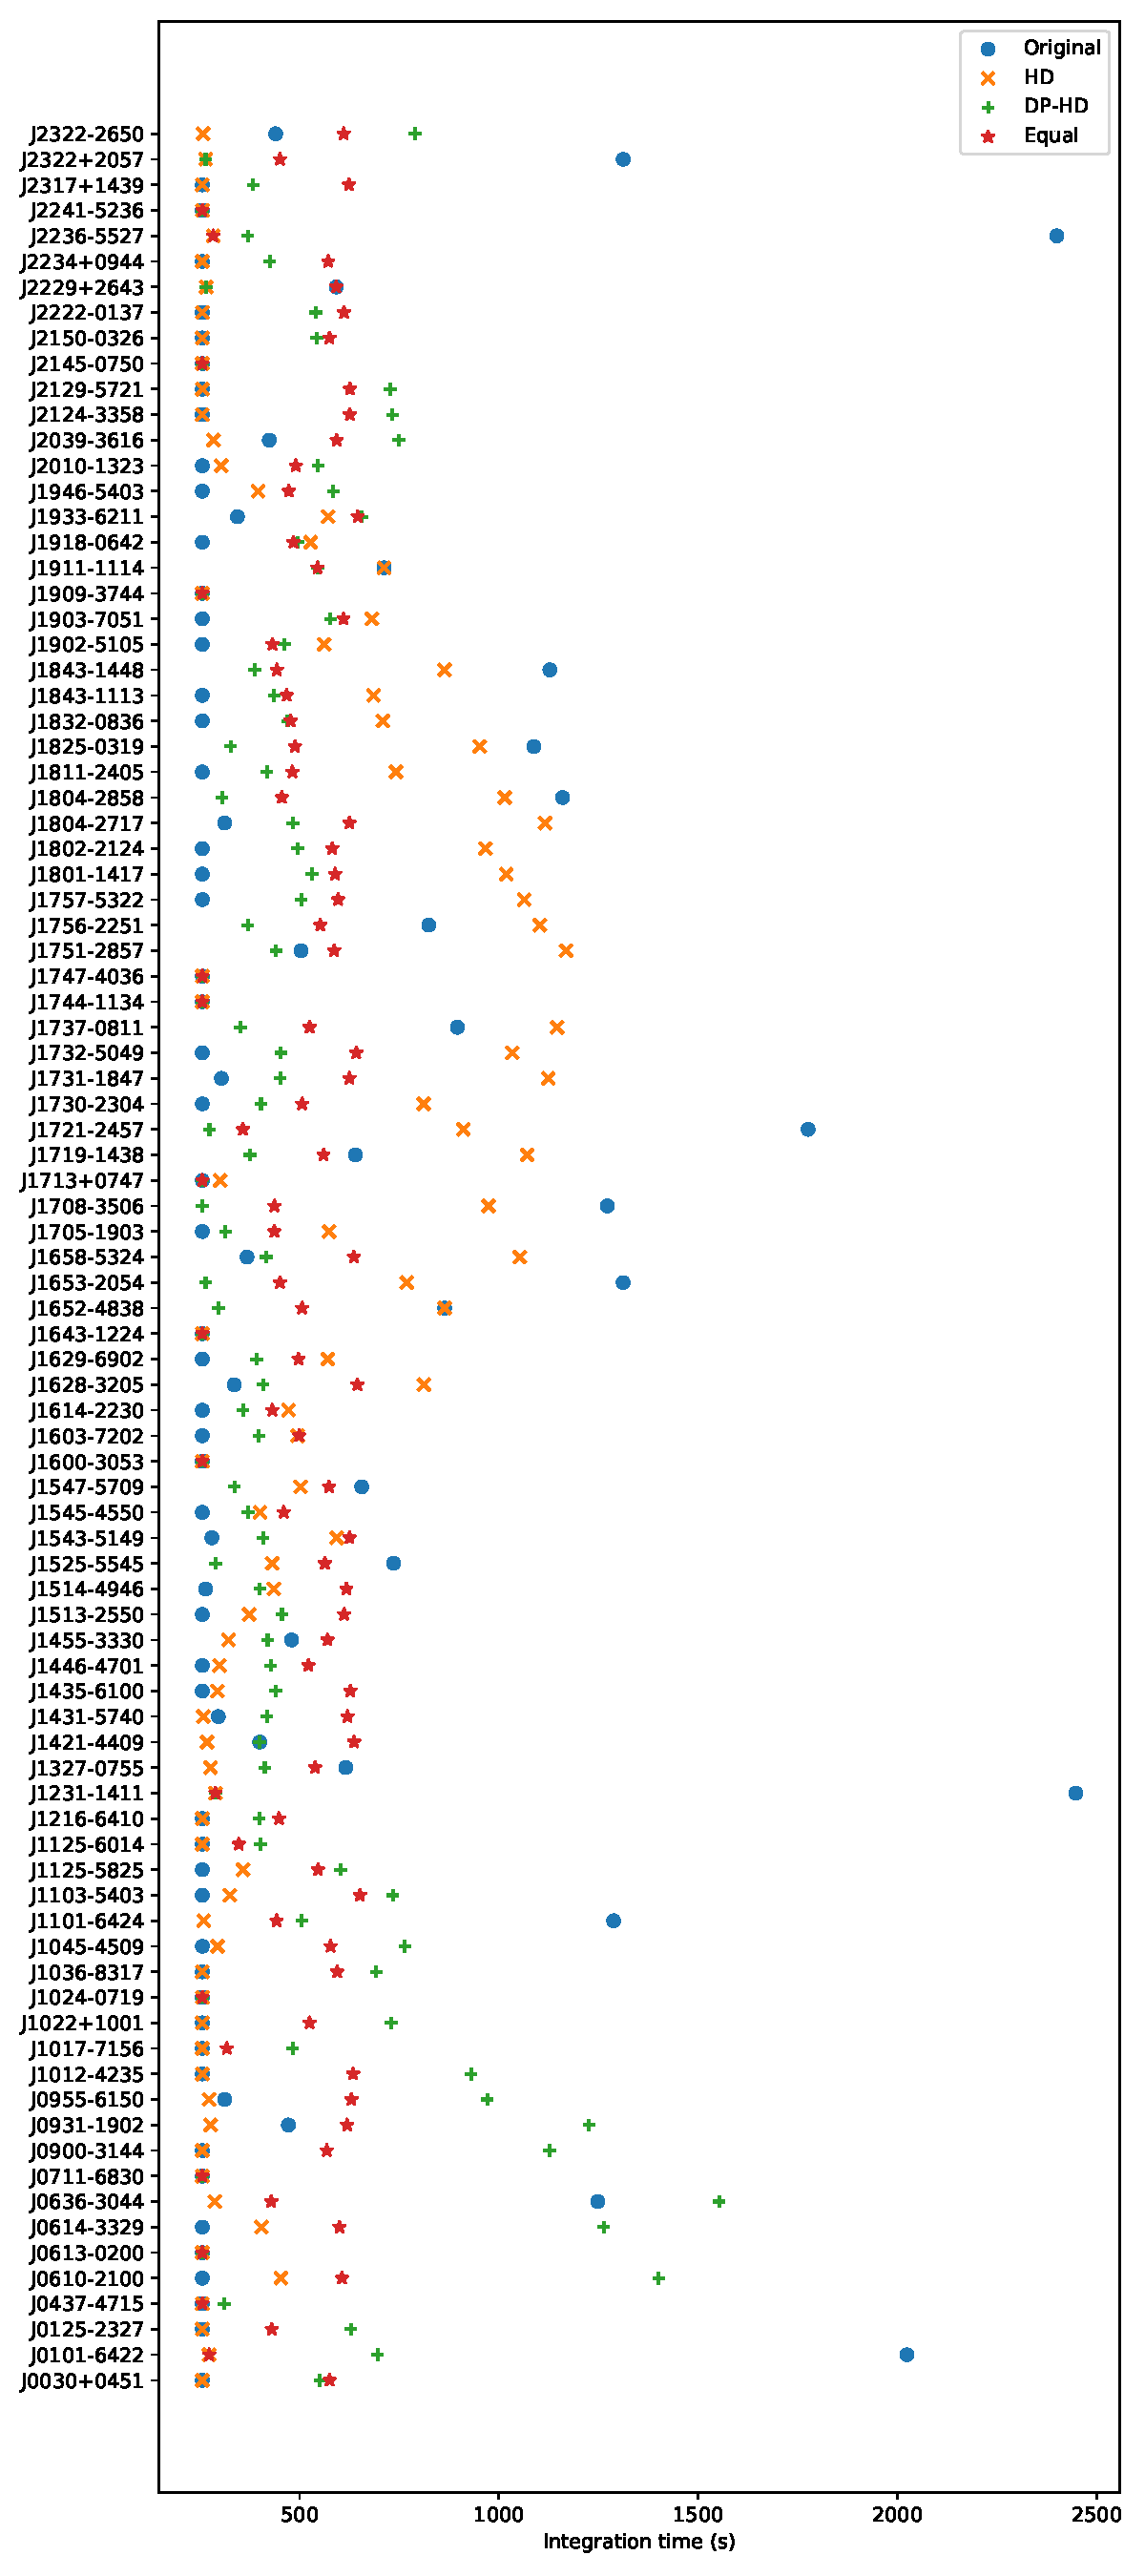
\includegraphics[width=0.57\textwidth]{./images/timeComparison.pdf}
\caption{\label{fig:obsTimes}
Integration times for each pulsar. 
Original times are shown as blue-circle markers. 
The other markers show integration times computed using different correlation functions for the time reallocation where Hellings-Downs, dipole minus Hellings-Downs, and equal are shown by orange-cross, green-plus, and red-star markers, respectively.
}
\end{figure*}

\begin{figure*}
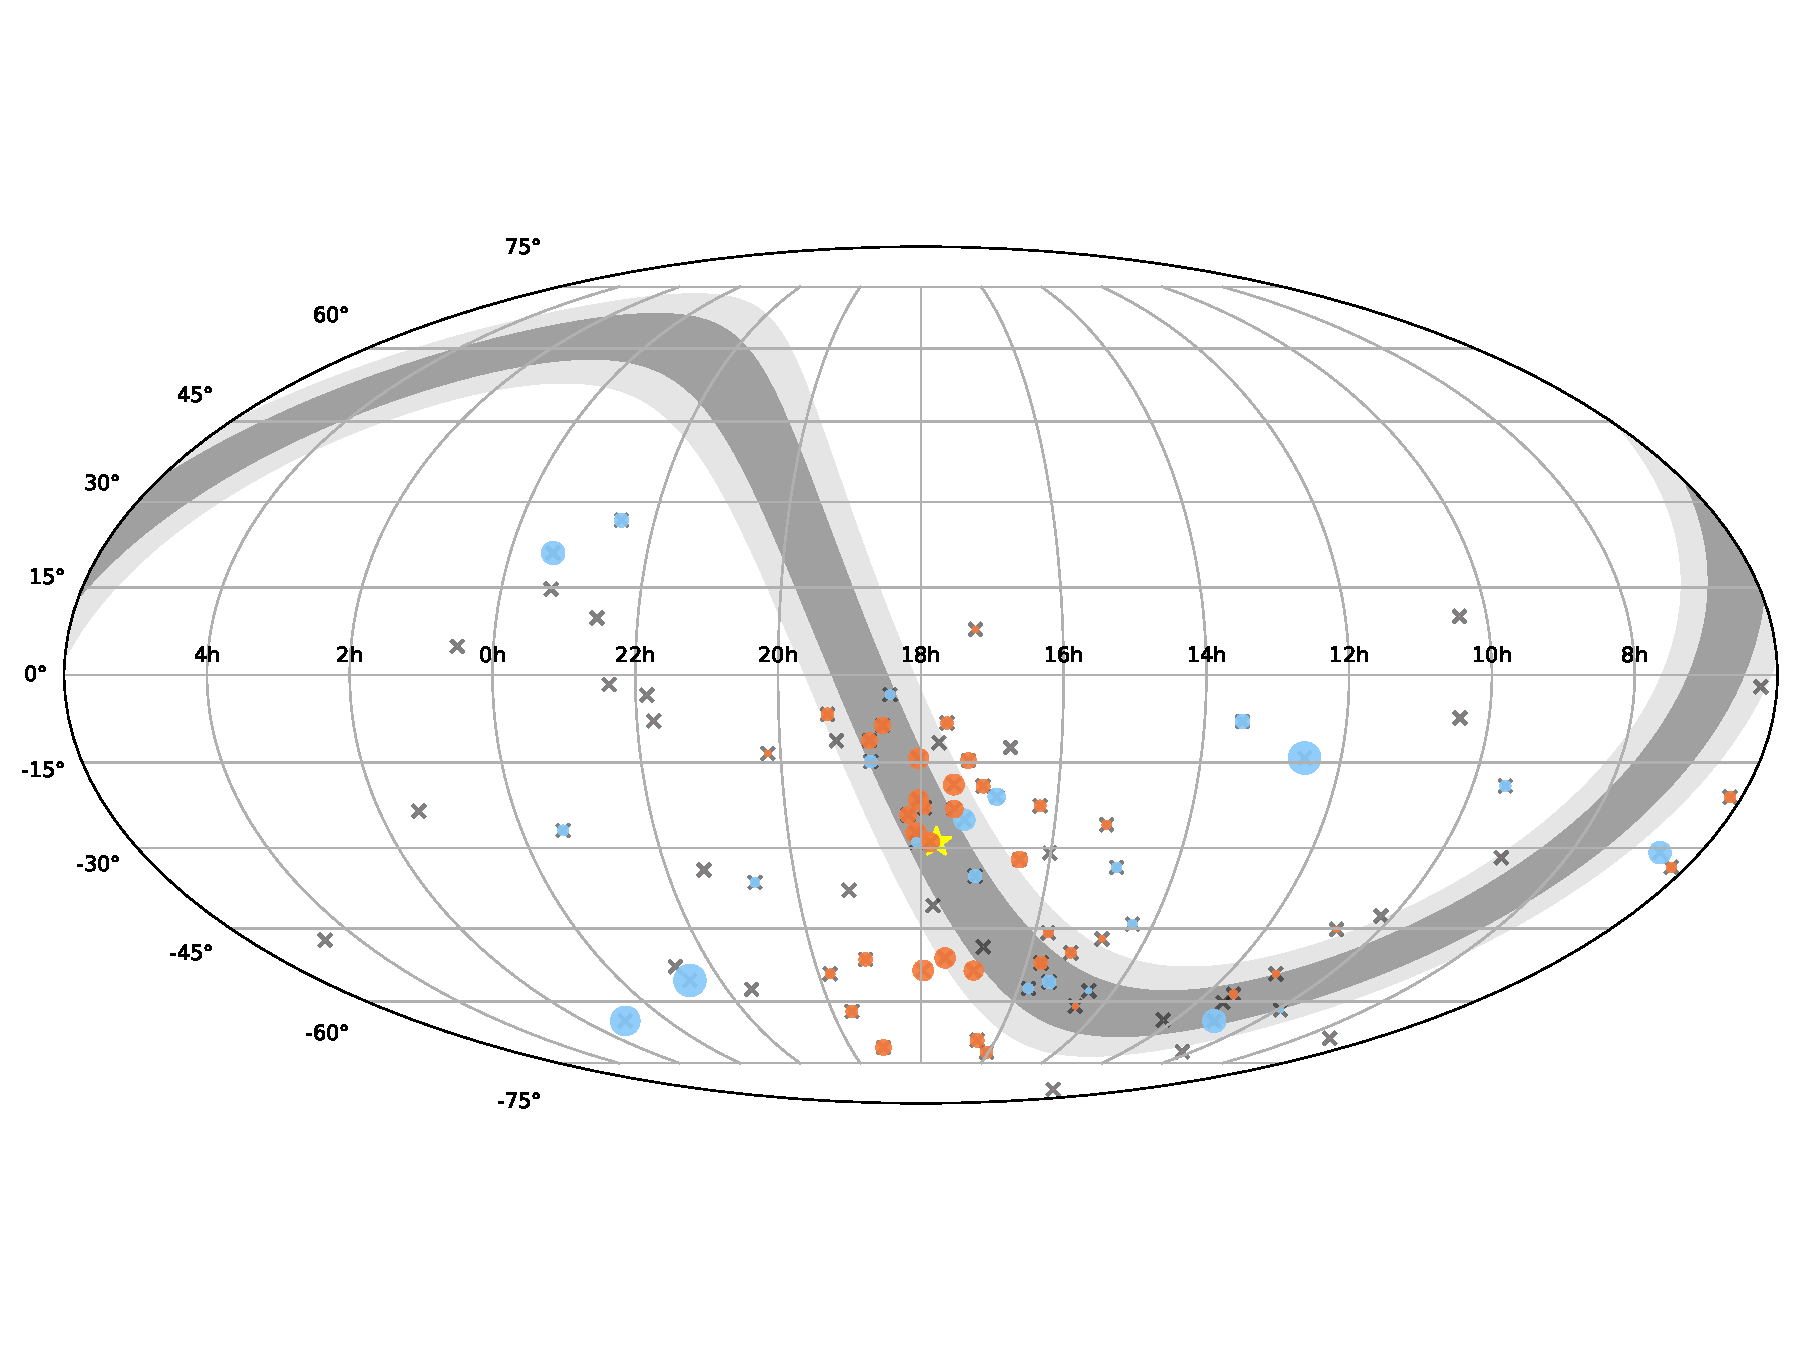
\includegraphics[trim={0cm 1cm 0cm 2cm},clip,width=0.8\textwidth]{./images/skymapHD.pdf}
\caption{\label{fig:skyHD}
Changes to integration times after time reallocation using the Hellings-Downs correlation. 
Each cross marker indicates a pulsar position on the sky. 
Orange and blue circles indicate pulsars that have gained and lost integration time as a result of the time reallocation. 
The size of the circle is proportional to the change in integration time. 
The yellow star and gray band indicate the galactic centre and galactic plane, respectively. 
Pulsars in the galatic centre generally gain more integration time due to the shape of the Hellings-Downs function as discussed in Section~\ref{sec:timeshuffle}.
}
\end{figure*}

\begin{figure*}
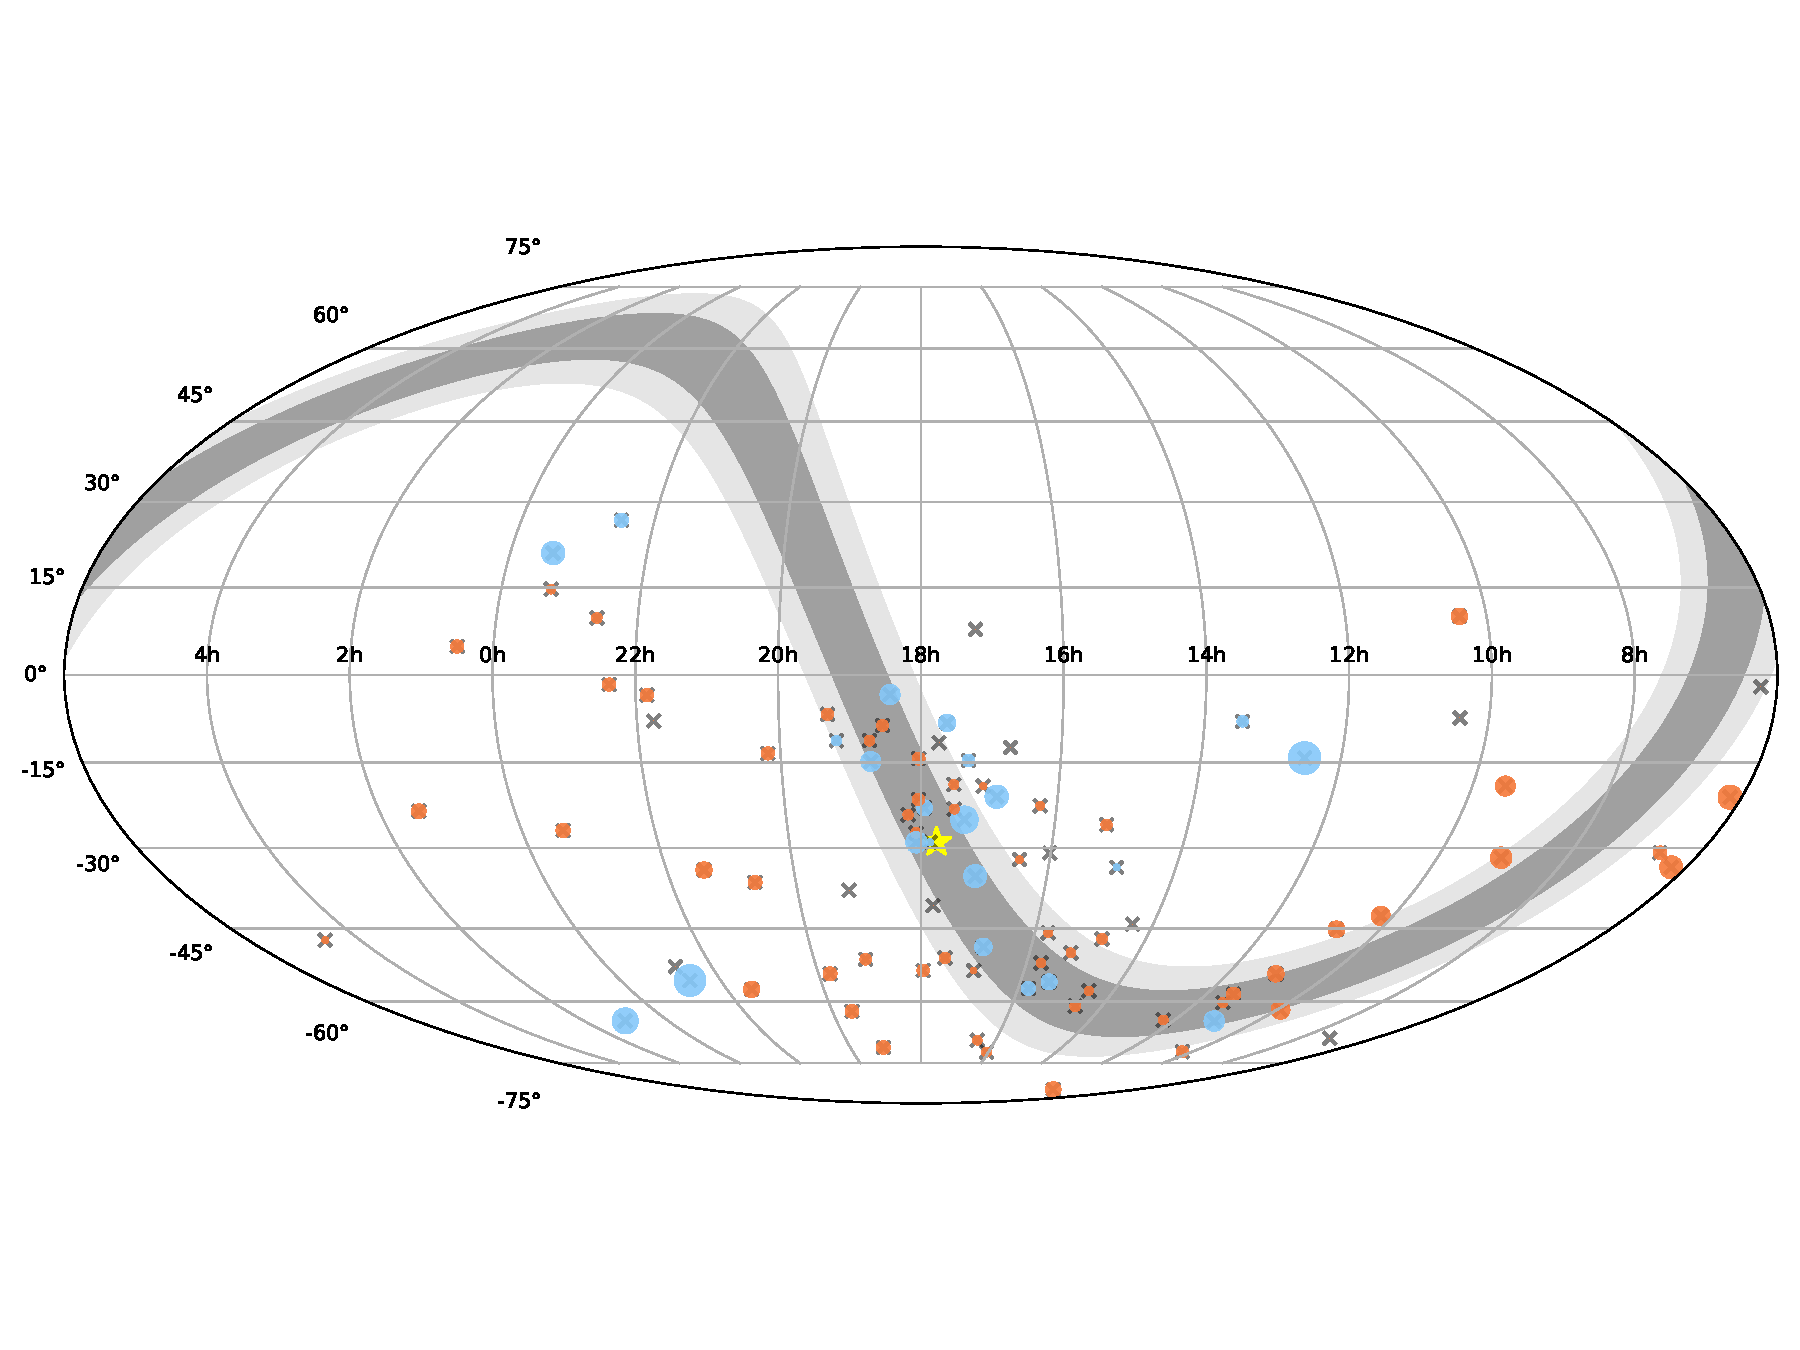
\includegraphics[trim={0cm 1cm 0cm 2cm},clip,width=0.8\textwidth]{./images/skymapDPHDDiff.pdf}
\caption{\label{fig:skyDPHDDiff}
Identical to Fig.~\ref{fig:skyHD} expect that the correlation function described in equation~\ref{eqn:chimod} is used to do the time reallocation calculation. 
Compared to Fig.~\ref{fig:skyHD}, integration time gains are more evenly spread across the sky. 
}
\end{figure*}

\begin{figure*}
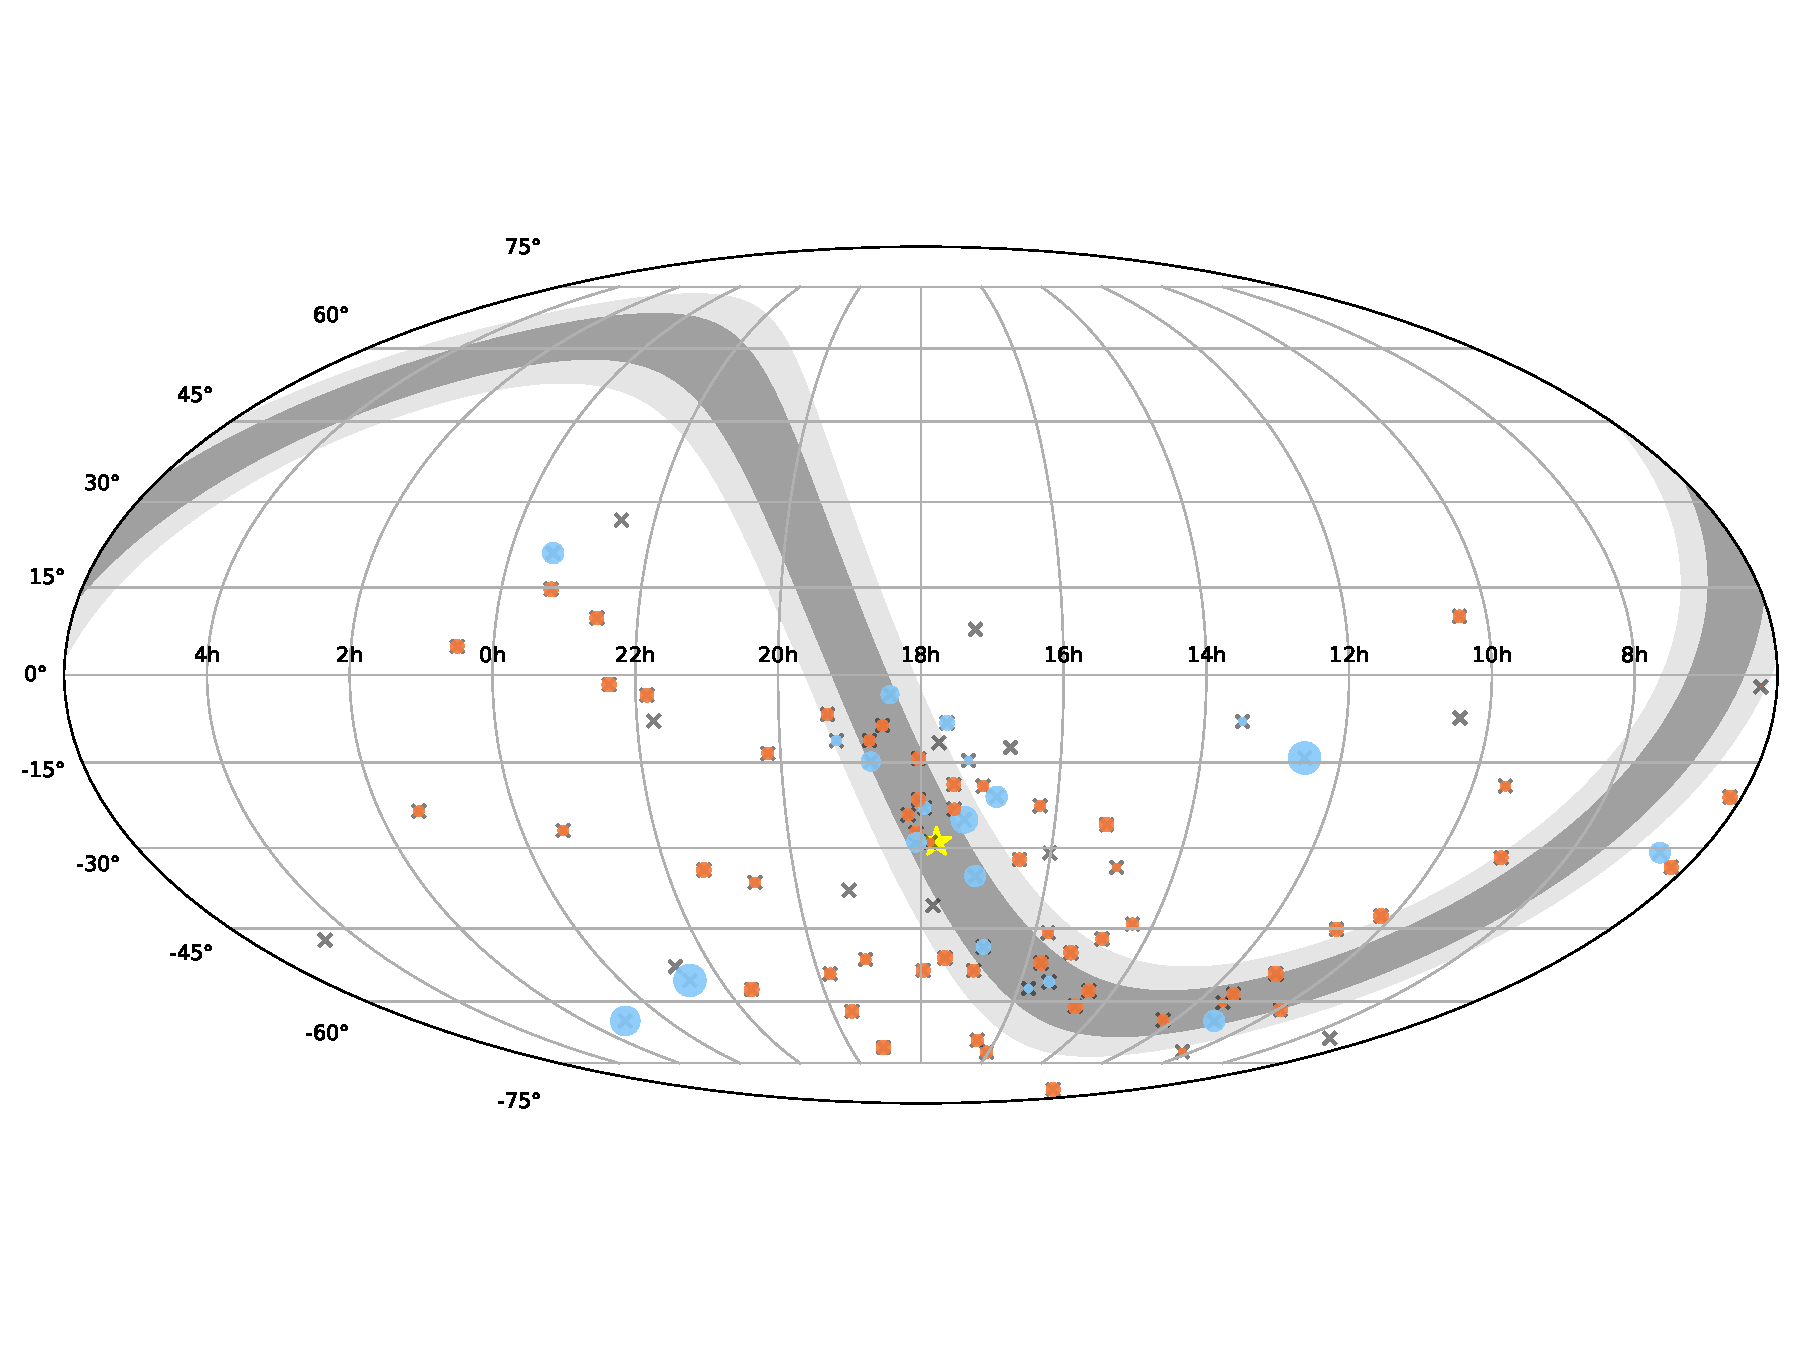
\includegraphics[trim={0cm 1cm 0cm 2cm},clip,width=0.8\textwidth]{./images/skymapEqual.pdf}
\caption{\label{fig:skyEqual}
Identical to Fig.~\ref{fig:skyHD} expect that an equal valued correlation function (across all anglular separtions) is used for the time reallocation. 
Similar to Fig.~\ref{fig:skyDPHDDiff}, the integration time gains are no longer concentrated in the galactic centre. 
}
\end{figure*}


\begin{figure*}
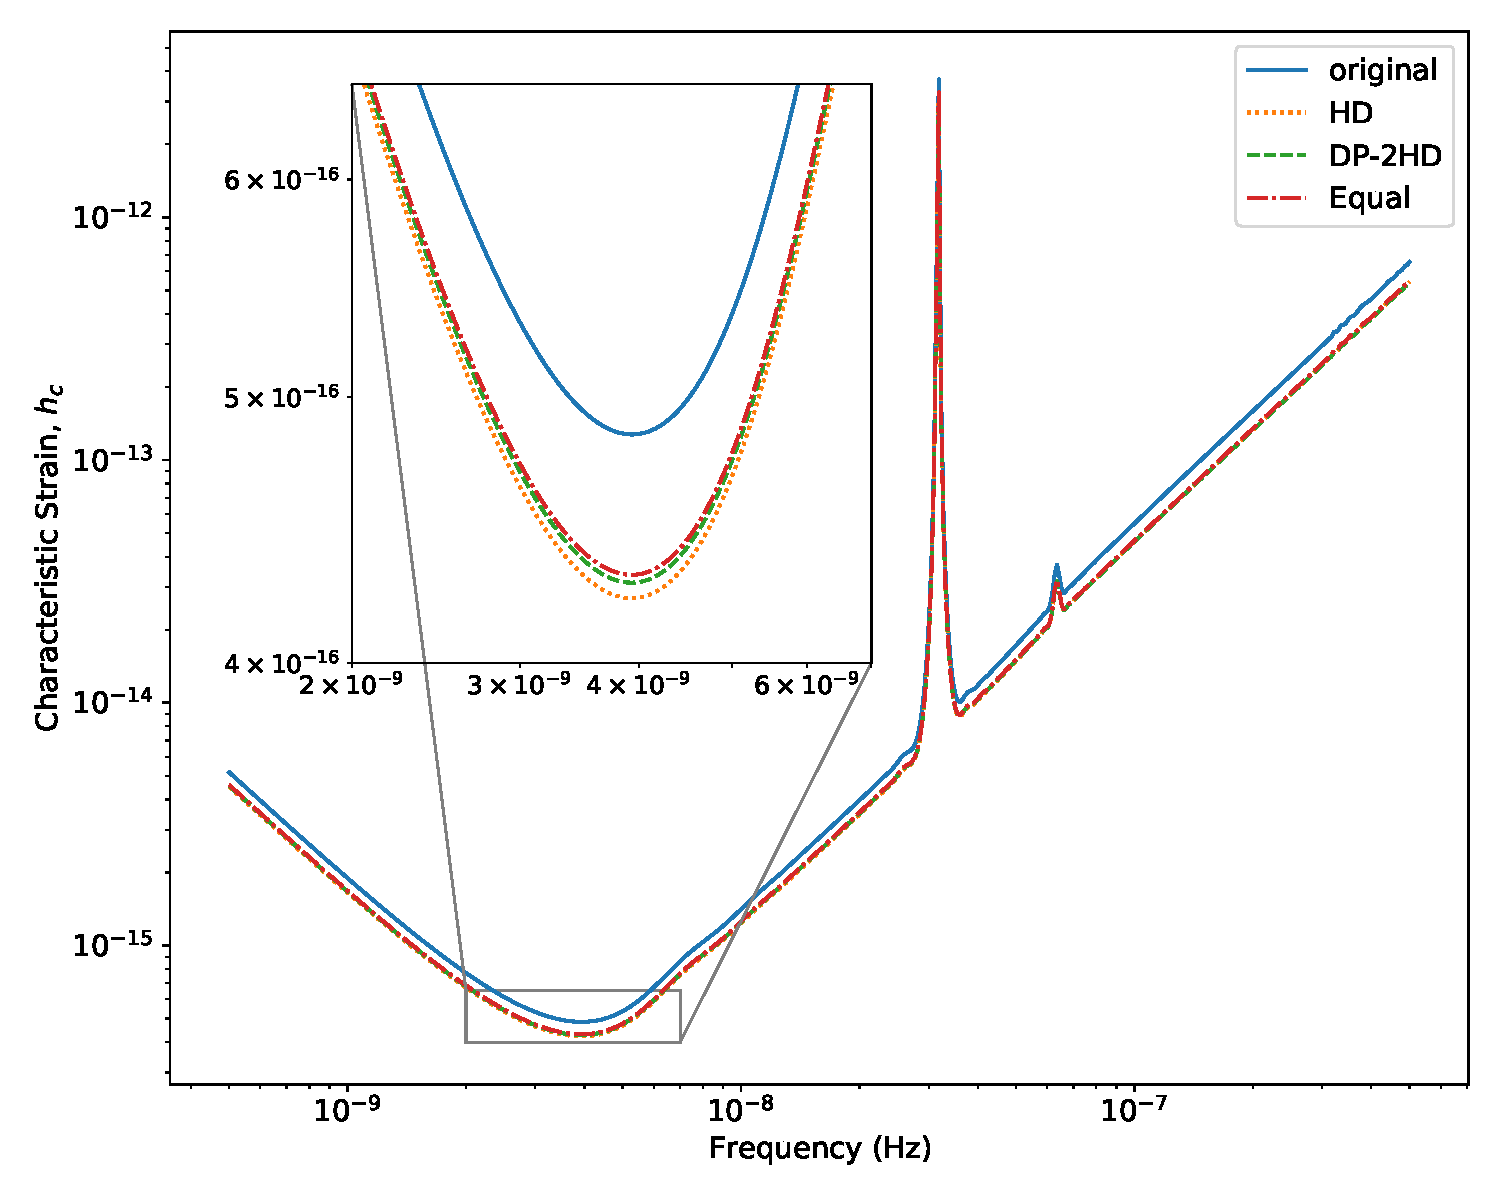
\includegraphics[width=0.8\textwidth]{images/hasasiaShuffle.pdf}
\caption{\label{fig:hasasiaShuffle}
PTA sensitivity curves for reallocation results using \texttt{hasasia}.
The original observing schedule is shown by the blue-solid line. 
Timing reallocation results using HD, DPHD, and Equal correlation functions are shown by the orange-dot, green-dash, and red-dot-dash lines, respetively. 
The inset show a zoom of the most sensitive frequencies. 
}
\end{figure*}

